% ------------------------------------------------------------
% Khảo sát dữ liệu nguồn (EDA) — bổ sung Chương 4, liên hệ Mục 2.2
% Hình: ../data/eda_output/figures/ (sinh bởi python -m data.run_preprocessing_eda)
% ------------------------------------------------------------
\subsection{Khảo sát và tìm hiểu dữ liệu nguồn}
\label{subsec:eda_source}

Trước khi chạy ETL, nhóm thực hiện \textbf{khảo sát dữ liệu thô} trên tập \texttt{flights.csv}
(kèm \texttt{airlines.csv}, \texttt{airports.csv}) nhằm đánh giá chất lượng, phát hiện giá trị thiếu
và ngoại lệ, đồng thời quan sát tương quan giữa các biến số --- phù hợp với khung tiền xử lý
đã trình bày ở Mục~2.2. Việc này giúp \textbf{minh chứng hóa} các quyết định làm sạch trong mã nguồn
\texttt{etl/transform.py} (điền \texttt{NaN} các cột delay bằng 0) thay vì chỉ dừng ở mô tả lý thuyết.

\subsubsection{Dữ liệu và phương pháp khảo sát}

Nguồn chính là bản ghi chuyến bay năm 2015 (định dạng CSV), gồm các nhóm thuộc tính:
thời gian lịch trình và thực tế, độ trễ cất cánh/đến, thời gian bay và quãng đường,
các thành phần trễ (NAS, hãng, tàu bay đến muộn, an ninh, thời tiết), cờ hủy chuyến và chuyển hướng.
Do kích thước tệp lớn ($\approx$\,5{,}8 triệu dòng), khảo sát định lượng được thực hiện trên
\textbf{mẫu 300\,000 dòng đầu} (đọc tuần tự từ đầu tệp) bằng script
\texttt{data/run\_preprocessing\_eda.py}, với các thống kê sau:
(i)~tỷ lệ thiếu và số quan sát ngoài rào \textbf{IQR bội số 1{,}5} (Tukey) trên từng cột số;
(ii)~ma trận tương quan Pearson giữa các biến liên tục;
(iii)~histogram mật độ \textbf{trước} làm sạch (giữ nguyên \texttt{NaN} khi vẽ phía ``trước'') và
\textbf{sau} khi áp dụng cùng quy tắc \texttt{to\_numeric(..., errors="coerce").fillna(0.0)}
cho các cột delay như trong luồng ETL.

\textit{Lưu ý:} Tỷ lệ thiếu và phân phối có thể thay đổi nhẹ nếu đổi cỡ mẫu hoặc dùng tùy chọn
\texttt{--only-operated} (lọc \texttt{CANCELLED=0}); khi cập nhật báo cáo, nên chạy lại script và
thay số trong bảng nếu cần.

\subsubsection{Giá trị thiếu và ngoại lệ (IQR)}

Bảng~\ref{tab:eda_outliers_summary} tóm tắt một số cột đo lường quan trọng.
Cột ``\% ngoài IQR'' là tỷ lệ quan sát \emph{có giá trị hợp lệ} nằm ngoài khoảng
$[Q_1 - 1{,}5\cdot\mathrm{IQR},\, Q_3 + 1{,}5\cdot\mathrm{IQR}]$.
Đối với \texttt{DEPARTURE\_DELAY} và \texttt{ARRIVAL\_DELAY}, tỷ lệ ngoài rào tương đối cao
phản ánh \textbf{đuôi phân phối dài} (một số chuyến trễ rất nhiều phút) --- đặc thù lĩnh vực hàng không,
không nhất thiết coi toàn bộ là lỗi đo; trong dự báo delay, các mô hình cây/GD thường xử lý tốt kiểu phân phối này.

Các cột phân tách nguyên nhân trễ (\texttt{AIR\_SYSTEM\_DELAY}, \texttt{AIRLINE\_DELAY}, \ldots)
có \textbf{khoảng 76\%} giá trị thiếu trên mẫu: đây là hiện tượng \emph{đặc thù dữ liệu nguồn}
(khi không ghi nhận chi tiết thành phần, ô để trống), không phải lỗi ngẫu nhiên toàn bảng.
Pipeline ETL quy ước điền 0 cho các cột delay (kể cả thành phần) để đồng nhất kiểu dữ liệu và phục vụ tổng hợp OLAP.

\begin{table}[H]
\centering
\caption{Khảo sát mẫu 300\,000 dòng \texttt{flights.csv}: thiếu và tỷ lệ ngoài rào IQR (Tukey, hệ số 1{,}5)}
\vspace{4pt}
\small
\setlength{\tabcolsep}{5pt}
\begin{tabular}{|l|r|r|r|}
\hline
\textbf{Cột} & \textbf{Tỷ lệ thiếu (\%)} & \textbf{\% ngoài IQR*} & \textbf{Ghi chú ngắn} \\ \hline
\texttt{DEPARTURE\_DELAY}   & 1{,}81  & 12{,}01 & Đuôi phân phối dài, nhiều chuyến trễ lớn \\ \hline
\texttt{ARRIVAL\_DELAY}     & 2{,}12  & 9{,}17  & Tương tự độ trễ đến \\ \hline
\texttt{ELAPSED\_TIME}      & 2{,}12  & 4{,}51  & Thiếu thường gắn chuyến chưa hoàn tất/hủy \\ \hline
\texttt{AIR\_TIME}          & 2{,}12  & 4{,}83  & Cùng nhóm thời gian bay \\ \hline
\texttt{DISTANCE}           & 0{,}00  & 5{,}80  & Một số quãng rất dài so với phần lớn \\ \hline
\texttt{SCHEDULED\_DEPARTURE} & 0{,}00 & 0{,}00  & Ít outlier theo IQR (phút trong ngày) \\ \hline
\texttt{Thành phần delay**} & $\approx$76 & --- & Thiếu khi không có chi tiết; ETL: \texttt{fillna(0)} \\ \hline
\end{tabular}
\\[4pt]
\footnotesize
*Trên các quan sát không thiếu của từng cột. **Nhóm \texttt{AIR\_SYSTEM\_DELAY}, \texttt{SECURITY\_DELAY},
\texttt{AIRLINE\_DELAY}, \texttt{LATE\_AIRCRAFT\_DELAY}, \texttt{WEATHER\_DELAY} có cùng mức thiếu trên mẫu.
\label{tab:eda_outliers_summary}
\end{table}

Bảng đầy đủ theo từng cột (kèm trung bình, độ lệch chuẩn, rào dưới/trên và tỷ lệ $|\mathrm{z}|>3$)
được xuất tự động ra tệp \texttt{data/eda\_output/outliers\_summary.csv} để tra cứu thêm.

\subsubsection{Ma trận tương quan giữa các biến số}

Hình~\ref{fig:eda_corr_heatmap} cho thấy mức độ tuyến tính Pearson giữa các biến liên tục trên cùng mẫu.
Các cặp như độ trễ cất cánh---độ trễ đến, thời gian lịch trình và các chỉ số thời gian bay có tương quan dương đáng kể,
phù hợp với vai trò của các đặc trưng thời gian và quãng đường trong mô hình dự báo
(Mục~\ref{subsec:chap4_mining}).
Ma trận này chỉ mang tính \textbf{mô tả}; quan hệ thực tế có thể phi tuyến và có tương tác theo hãng/sân bay/tháng.

\begin{figure}[H]
    \centering
    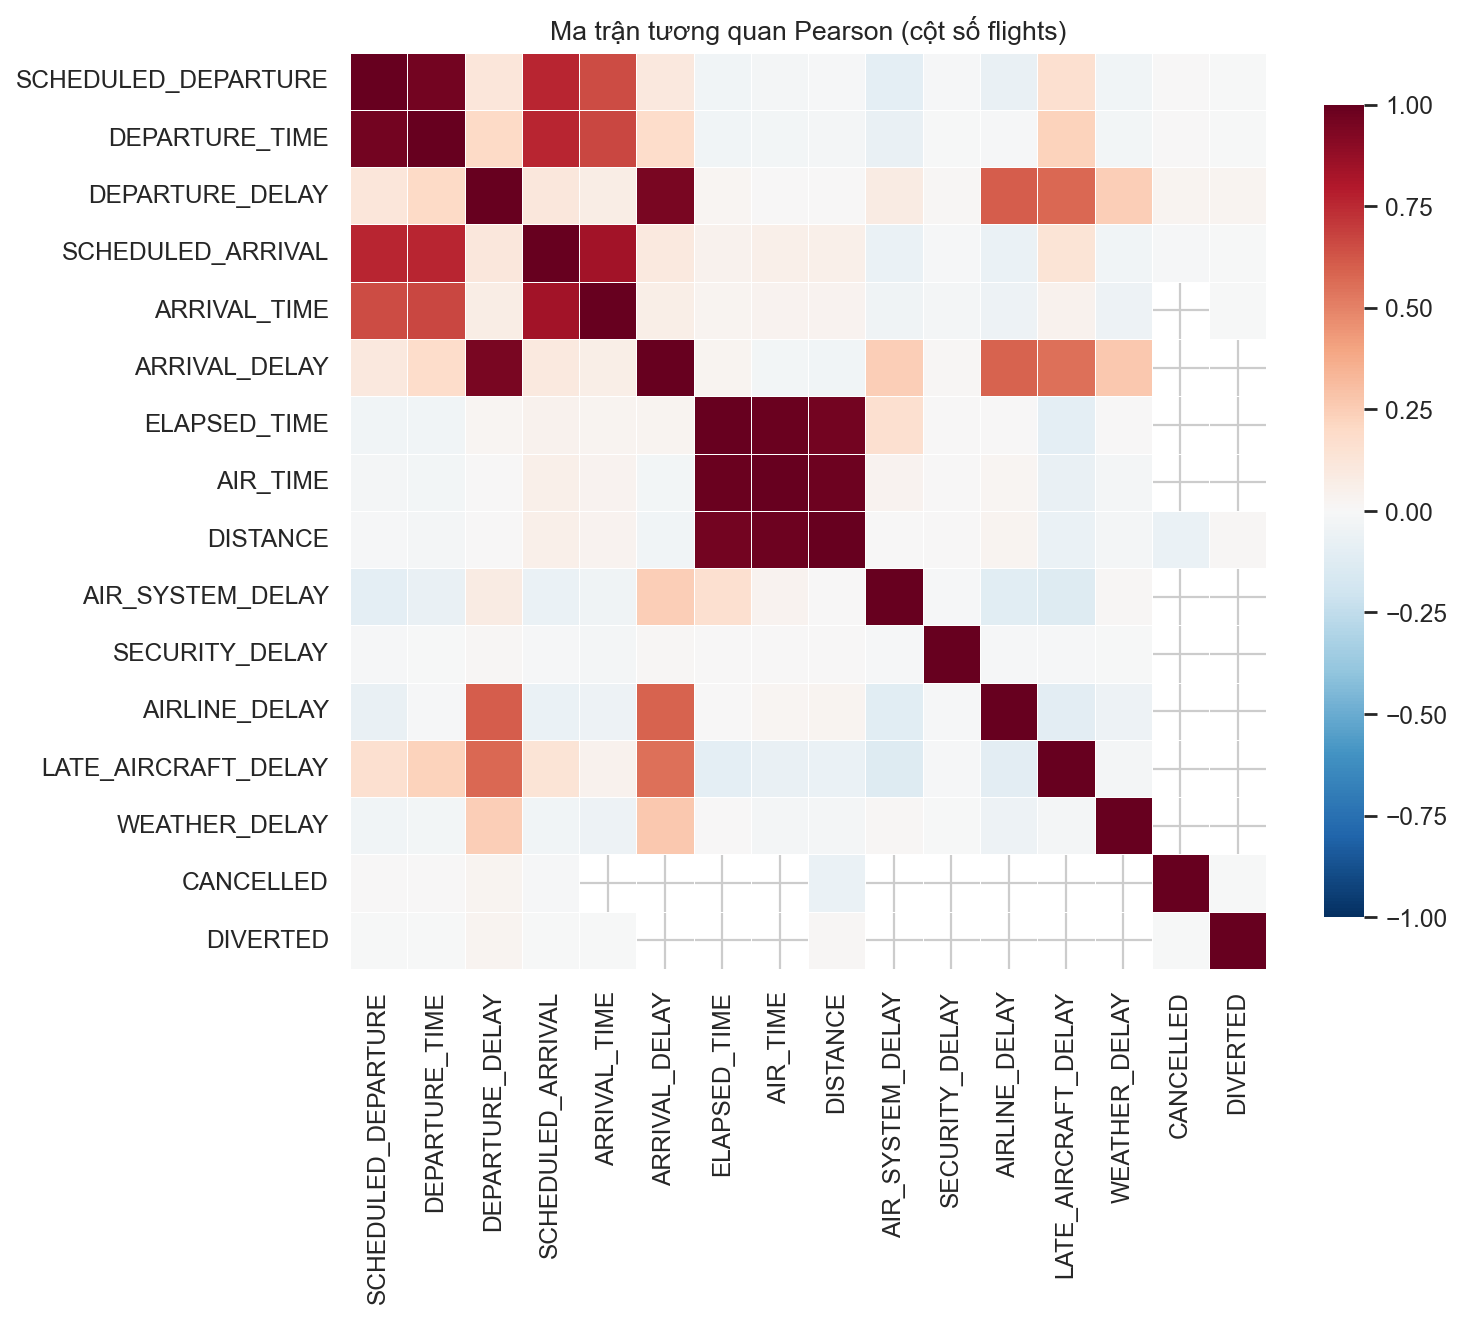
\includegraphics[width=0.95\textwidth]{../data/eda_output/figures/correlation_heatmap.png}
    \caption{Heatmap tương quan Pearson trên mẫu 300\,000 dòng (các cột số có trong \texttt{flights.csv}).}
    \label{fig:eda_corr_heatmap}
\end{figure}

\subsubsection{Phân phối trước và sau bước làm sạch delay}

Hình~\ref{fig:eda_delay_before_after_dep} và Hình~\ref{fig:eda_delay_before_after_arr} so sánh
mật độ xác suất ước lượng bằng histogram (trục hoành clip trong khoảng hẹp để dễ so sánh \emph{hình dạng}
phần khối lượng lớn; phần đuôi cực đại vẫn được phản ánh ở bảng outlier).
\textbf{Trước:} phân phối trên quan sát không thiếu, thể hiện khối lượng lớn tại vùng trễ nhỏ và ít
giá trị thiếu (tỷ lệ ghi trên hình). \textbf{Sau:} cùng dữ liệu sau khi gán 0 cho \texttt{NaN} ở các cột delay
như trong \texttt{transform\_chunk} --- các ô thiếu trở thành khối tại 0, phản ánh quy ước nghiệp vụ
``không ghi nhận độ trễ $\rightarrow$ coi như 0'' trong pipeline kho dữ liệu.

\begin{figure}[H]
    \centering
    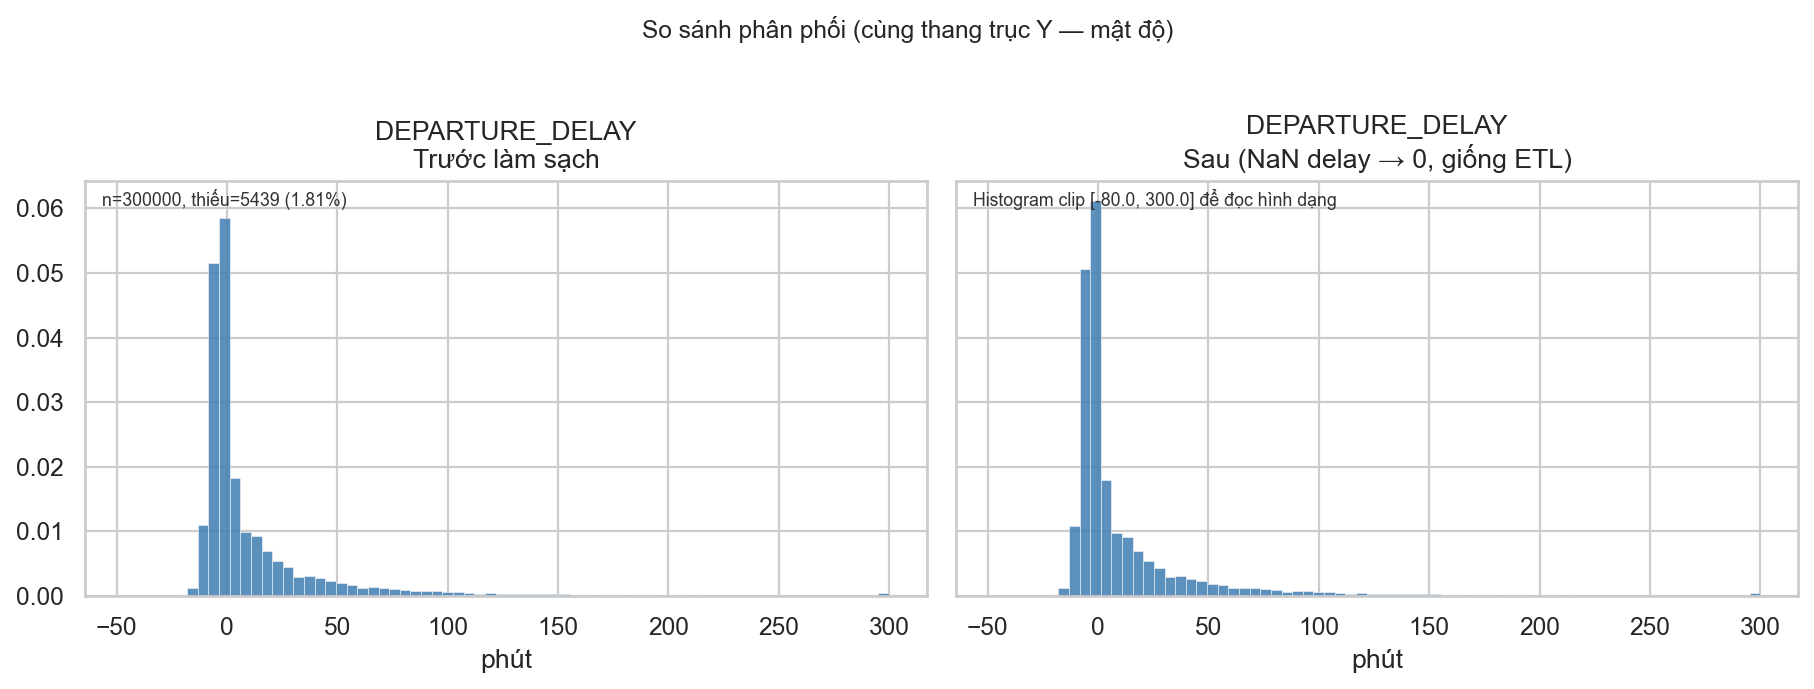
\includegraphics[width=0.95\textwidth]{../data/eda_output/figures/delay_before_after_departure_delay.png}
    \caption{Phân phối \texttt{DEPARTURE\_DELAY}: trước làm sạch (trái) và sau khi \texttt{NaN} $\rightarrow$ 0 (phải), mẫu 300\,000 dòng.}
    \label{fig:eda_delay_before_after_dep}
\end{figure}

\begin{figure}[H]
    \centering
    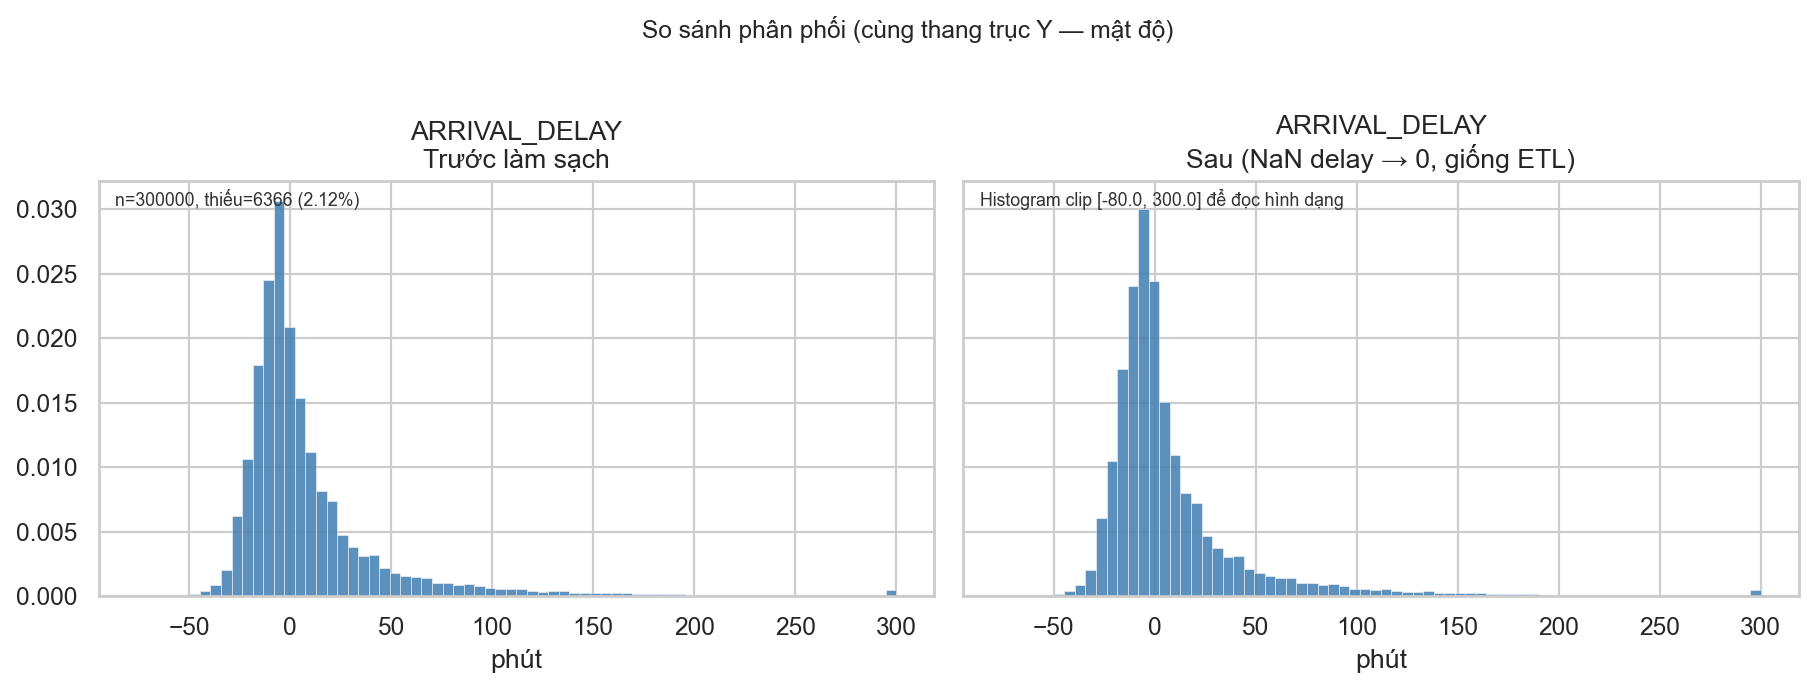
\includegraphics[width=0.95\textwidth]{../data/eda_output/figures/delay_before_after_arrival_delay.png}
    \caption{Phân phối \texttt{ARRIVAL\_DELAY}: trước và sau làm sạch delay (cùng mẫu và quy tắc như Hình~\ref{fig:eda_delay_before_after_dep}).}
    \label{fig:eda_delay_before_after_arr}
\end{figure}

\subsubsection{Kết luận ngắn gọn}

Khảo sát cho thấy dữ liệu nguồn có \textbf{thiếu có cấu trúc} (đặc biệt delay thành phần và một số thời điểm thực tế)
và \textbf{đuôi nặng} trên các biến trễ; các bước làm sạch trong ETL (chuẩn hóa kiểu, điền 0 cho nhóm delay,
loại bản ghi không map được khóa chiều) là phù hợp với đặc điểm thống kê quan sát được và với lý thuyết tiền xử lý ở Chương~2.
